%% The following is a directive for TeXShop to indicate the main file
%%!TEX root = diss.tex
\chapter{Fair contribution valuation in vertical federated
learning}
\label{ch:Val-VFL}

\section{Introduction} \label{sec:8-1}
As we introduced in \autoref{ch:Val-HFL}, the effectiveness of federated
learning (FL) depends on the active participation of motivated clients. Because fair cooperation and reward can motivate clients' participation, it is vital to understand how to fairly and effectively evaluate clients' contributions. In this chapter, we concentrate on developing efficient and equitable methods for evaluating clients' contributions in vertical federated learning (VFL) systems.

Recall that the Shapley value is the only metric that satisfies all four requirements of Shapley's fairness criteria: \emph{balance}, \emph{symmetry}, \emph{zero element}, and \emph{additivity}~\cite{dubey1975uniqueness} (see \autoref{sec:8.4} for a quick review).  Although the Shapley value has many desirable characteristics, its evaluation in the FL context requires repeatedly training and evaluating a machine learning model on all possible subsets of clients. The corresponding communication and computational costs are exponential, and thus are often prohibitive in practice~\cite{song2019profit,wang2019measure,fan2021improving}. 

Variants of the Shapley value make equitable data owner contribution assessment feasible in FL. For HFL, Wang \textit{et al.}~\cite{wang2020principled} proposed a contribution valuation metric called federated Shapley value (FedSV). The key idea is to calculate Shapley values for clients in each round of training and then to report the sum of the Shapley values for all clients as the final results. Computation of the FedSV does not need model retraining and retains some, but not all, of Shapley's fairness criteria. Fan \textit{et al.}~\cite{fan2021improving} further improved the fairness of this approach by leveraging low-rank matrix factorization techniques. 

Relative to HFL, adapting the Shapley value to VFL faces another challenge because of the stronger model dependence in the vertical context. More precisely, the Shapley value computation requires us to form the model produced by all different subsets of clients. This requirement is easy to satisfy under HFL because the global model is defined as the additive aggregation of the local models and thus we only need to aggregate local models from different subsets of clients~\cite{wang2020principled}. In the vertical context, however, the global model is the concatenation of local models that are not shared with the server. Thus, simply concatenating local models from different subsets of clients does not work. 

 We propose a contribution valuation metric called the vertical federated Shapley value (VerFedSV)
where the clients' contributions are computed at multiple time points during the training process. We resolve the model concatenation problem by carefully utilizing clients' embeddings at different time-stamps. 
%See Section~\ref{sec:4} for a detailed discussion. 
We demonstrate that our design retains many desirable fairness properties and can be efficiently implemented without retraining. 

VFL algorithms can be divided into two categories: synchronous methods~\cite{Gong2016PrivateDA,Zhang2018FeatureDistributedSF,liu2019communication}, where periodic synchronizations
 among clients are required, and asynchronous ones
 ~\cite{Hu2019FDMLAC,Gu2020PrivacyPreservingAF,chen2020vafl}, where clients are allowed to conduct local computation asynchronously. We show that VerFedSV is applicable to both synchronous and asynchronous VFL settings. Under the synchronous setting, we show that FedSV can be computed by leveraging some matrix-completion techniques. Although there are many similarities between synchronous and asynchronous VFL settings, contribution valuation in an asynchronous VFL setting is more complicated because the contribution of a client not only depends on the relevance of the client's data to the training task, but also depends on the client's local computational resource. We demonstrate that our design can reflect the strength of clients' local computational resources under the asynchronous setting. To the best of our knowledge, we are the first to consider the contributions in local computational resources.

Our contributions can be summarized as follows.
\begin{enumerate}
    \item We propose vertical federated Shapley value (VerFedSV) for vertical federated learning (\autoref{def:vertical_fedsv}), which satisfies the desirable properties for fairness (\autoref{prop:fair}). 
    \item Under the synchronous vertical federated learning setting, we show that VerFedSV can be computed by solving low-rank matrix completion problems for embedding matrices, which are proven to be approximately low rank (\autoref{prop:low-rank}). We also give an approximation guarantee on VerFedSV given the tolerance for matrix completion (\autoref{prop:syn_verfedsv}).
    \item Under the asynchronous vertical federated learning setting, we show that VerFedSV can be directly computed and can indeed reflect the strength of clients' local computational resources (\autoref{prop:asyn_diff_fre}).
    \item We show that the computational complexity of VerFedSV can be further reduced by applying Monte-Carlo sampling methods (\autoref{sec:8.7}). 
\end{enumerate}

\section{Related work} \label{sec:8.2}

Shapley value~\cite{shapley201617} has had extensive applications in economics~\cite{gul1989bargaining}. Dubey~\cite{dubey1975uniqueness} showed that Shapley value is the unique measure that satisfies the four fundamental requirements of fairness proposed by Shapley~\cite{shapley201617}. Limited by space, here we restrict our discussion to Shapley-value-based valuation strategies related to machine learning. 

Ghorbani and Zou~\cite{ghorbani2019data} proposed the Shapely value-based metric for quantifying data contributions in machine learning. They introduced a data Shapley value metric for quantifying the contribution of a single data point to a learning task. They noted that directly computing the data Shapley value requires exponential-time complexity and suggested two heuristic approximation approaches to improve efficiency. Jia \textit{et al.}~\cite{jia2019towards} presented various efficient techniques for estimating the data Shapley value, including approaches based on group testing and compressed sensing. Ghorbani \textit{et al.}~\cite{ghorbani2020distributional} extended the notion of data Shapley value from a fixed training data set to arbitrary data distribution, called distributional Shapley value. Theoretically, they proved that their proposed measure is stable as similar distributions yield similar value functions. Kwon \textit{et al.}~\cite{kwon2021efficient} then developed analytic expressions for distributional Shapley value for several machine learning tasks, including linear regression and binary classification.

Song \textit{et al.}~\cite{song2019profit} introduced the concept of data Shapley value to HFL and proposed contribution index (CI). They pointed out that directly calculating CI requires retraining the model exponentially, which is costly in federated learning. They offered two gradient-based techniques to approximate the contribution index. Wang \textit{et al.}~\cite{wang2020principled} alternatively solved this problem by proposing a new measure for HFL, called federated Shapley value, which can be determined from local model updates in each training iteration. Federated Shapley value does not need model retraining and preserves some but not all of the favorable qualities of the traditional Shapley value. Fan \textit{et al.}~\cite{fan2021improving} further improved the fairness of this approach. 

Wang \textit{et al.}~\cite{wang2019measure} and more recently Han \textit{et al.}~\cite{han2021data} extended the notion of data Shapley value to VFL. As discussed before, the need of retraining the model for different subsets of clients is a bottleneck of Shapley value computation in federated learning. Both of these two works~\cite{wang2019measure,han2021data} solved this problem by introducing model-independent utility functions, where model-independency means that the contribution of a client does not depend on the performance of the final model, and thus does not require retraining of the model. In particular, Wang \textit{et al.}~\cite{wang2019measure} suggested using the situational importance (SI)~\cite{achen1982interpreting}, which computes the difference between the embeddings with true features and expected features. However, computing SI requires knowing the expectation of each feature and can be impractical under VFL. Han \textit{et al.}~\cite{han2021data} suggested to use the conditional mutual information (CMI)~\cite{brown2012conditional}, which computes the tightness between the label and features. However, computing CMI requires every client to access the labels, which may also be impractical under VFL and leak privacy. Besides the above shortcomings, the model-independent utility function itself may cause some fairness issues when the VFL is conducted asynchronously. As we discussed in \autoref{sec:8.1}, under the asynchronous setting, the contribution of a client not only is related to the quality of the local dataset but also depends on the power of local computational resources. Model-independent utility functions cannot fully reflect a client's contribution in this case. In this work, we instead use model-dependent utility function and resolve the requirement on retraining the model by periodically evaluating the Shapley during the training process.

\section{Vertical federated learning} \label{sec:8.3}
In this section, we revisit the VFL model. Consider the following standard VFL scenario: $M$ clients and a single server collaborate to train a machine learning model on $N$ data samples $\{(x_i \in \mathbb{R}^d, y_i \in \{\pm 1\})\}_{i=1}^N$, where $x_i$ is the feature vector and $y_i$ is the label. Let $[N] = \{1, \dots, N\}$ denote the set of all sample indices. 
Every feature vector $x_i$ is distributed across $M$ clients $\{x^m_i\in\mathbb{R}^{d^m}: m \in [M]\}$, where $d^m$ is the feature dimension for client $m$ such that $\sum_{m=1}^M d^m = d$ and $[M] = \{1,\dots, M\}$ denotes the set of all clients. The local data set for any client $m$ is
\[\mathcal{D}^m = \{x_i^m : i \in [N]\}.\]
The server maintains all the labels $\mathcal{D}^s = \{y_i: i \in [N]\}$. 
The collaborative training problem can be formulated as
\begin{equation} \label{eq:main_prob3}
    \min_{\theta_1, \dots, \theta_M} \enspace \frac{1}{N}\sum_{i=1}^N \ell\left(\theta_1, \dots, \theta_M; \{x_i, y_i\} \right),
\end{equation}
where $\theta_m \in \mathbb{R}^{d_m}$ denotes the training parameters of the $m$th client, $\ell(\cdot)$ denotes the loss function. For a wide range of models, such as linear and logistic regression, and support vector machines, the loss function has the form
\begin{equation} \label{eq:loss_function}
     \ell\left(\theta_1, \dots, \theta_M; \{x_i, y_i\} \right) 
     := 
     f\left( h_i; y_i\right)
\end{equation}
where 
\[h_i = \sum_{m=1}^M h_i^m, \enspace h_i^m = \langle \theta_m, x_i^m \rangle,\]
and $f(\cdot; y)$ is a differentiable function for any $y$. For each client $m$, the term $h_i^m$ can be viewed as the client's embedding of the local data point $x_i^m$ and the local model $\theta_m$. To preserve the privacy, clients are not allowed to share their local data set $\mathcal{D}^m$ or local model $\theta^m$ with other clients or with the server. Instead, clients can share only their local embeddings $\{h_i^m\mid i\in[N]\}$ to the server for training. 

For simplicity, here we consider a binary classification problem. All our theoretical results can be easily extended to a multiclass classification problem with $l > 2$ classes, where $\theta_m \in \mathbb{R}^{d_m \times l}$ and $h_i^m = \theta_m^\intercal x_i \in \mathbb{R}^l$. Moreover, in practice, our method also works for more general local embedding functions, i.e., $h_i^m = g(\theta_m; x_i^m)$, where $g$ can be a neural network with weights $\theta_m$. We empirically verify this in Section 8.

The communication between the server and the clients is widely recognised as the primary bottleneck in federated learning. Each cycle of communication consists of an upload and a download. We follow Dinh \textit{et al.}~\cite{dinh2020federated} and assume that  download times are negligible in comparison to upload times. This assumption is reasonable because downlinks typically occur over large bandwith channels, and the power of the edge server is much more than the transmission power of the client. We introduce the following definition to quantify the strength of clients' local computational resources.

\begin{definition} \label{def:communication}
    Let $\Delta t > 0$ be the unit time for any communication round. The strength of each client $m$'s local computational resources is represented by a positive integer $\tau_m \in [1, N]$, such that client $m$ can compute and upload at most $\tau_m$ local embeddings during each time interval $\Delta t$. 
\end{definition}

In this chapter, we use the notions of several special classes of functions, i.e., strongly convex and Lipschitz and smooth, and notions of $\epsilon$-net and covering number, which are tools widely used in high-dimensional probability~\cite{vershynin2018high}. Due to the page limit, we include the formal definitions of these notions in the supplementary material.

\section{Vertical federated Shapley value} \label{sec:8.4}
Fairness is one of the most desirable properties for a contribution valuation metric \cite{ghorbani2019data,pei2020survey}. Under the FL setting, a contribution valuation metric should reflect how much each client contributes to the performance of the final model. Formally, we assume a black-box utility function $U:2^{[M]} \to \mathbb{R}$ such that for any subset of clients $S \subseteq [M]$, the function $U(S)$ returns a utility score of the model collaboratively trained by the clients in $S$, such as the performance of the model. Let $v: [M] \to \mathbb{R}$ be the evaluation metric associated with the utility function $U$. Given the utility function $U$, the Shapley fairness criteria~\cite{shapley201617} has four fundamental requirements for any metric $v$.
\begin{enumerate}
    \item \textbf{Symmetry.} For any two clients $i, j \in [M]$, if for any subset of clients $S \subseteq [M] \setminus \{i,j\}$, $U(S \cup \{i\}) = U(S \cup \{j\})$, then $v(i) = v(j)$. 
    \item \textbf{Zero element.} For any client $i \in [N]$, if for any subset of clients $S \subseteq [M] \setminus \{i\}$, $U(S \cup \{i\}) = U(S)$, then $v(i) = 0$.
    \item \textbf{Additivity.} If the utility function $U$ can be expressed as the sum of separate utility functions, namely $U = U_1 + U_2$ for some $U_1, U_2 : 2^I \to \mathbb{R}$, then for any client $i \in [M]$, $v(i) = v_1(i) + v_2(i)$, where $v_i$ and $v_2$ are the evaluation metrics associated with the utility functions $U_1$ and $U_2$, respectively. 
    \item \textbf{Balance.}  $U([M]) = \sum_{i \in [M]} v(i)$.
\end{enumerate}
Note that, although balance is a necessary condition in many economic contests because it ensures payment is fully distributed to all clients, it is irrelevant in the context of our paper because we are only concerned about the relative contributions of clients. It has been shown that if the contribution valuation metric $v$ satisfies symmetry, zero element, and additivity, then $v$ must have the form
\begin{equation} \label{eq:shapley2}
    v(i) = c \sum\limits_{S \subseteq I \setminus\{i\}} \frac{1}{\binom{N-1}{|S|}} \left[U(S\cup\{i\}) - U(S)\right]
\end{equation}
for some positive constant $c$~\cite{dubey1975uniqueness,ghorbani2019data}. However, the contribution valuation metric in~\eqref{eq:shapley} is impractical in the federated learning context because the evaluation of the utility function $U$ requires retraining models~\cite{ghorbani2019data,wang2020principled}. To make a fair evaluation of data owners computationally practical in federated learning, as discussed before, Wang \textit{et al.}~\cite{wang2020principled} recently proposed the federated Shapley value (FedSV) for HFL, which computes the Shapley values for clients periodically during the training and then reports the summation over all the periods as the final results. We extend this idea to the VFL context. 

Suppose we pre-determine $T$ time-stamps for contribution valuation and use $[T] = \{1,\dots, T\}$ to denote the set of all time-stamps. At each time $t \in [T]$, we define the utility function $U_t:2^{[M]}\to\mathbb{R}$ such that for any subset of clients $S \subseteq [M]$, the utility $U_t(S)$ denotes the decrease in loss made by the clients in $S$ during the time period $[t-1, t]$, i.e., 
\begin{align} \label{eq:utility2}
    U_t(S) = &~ \frac{1}{N} \sum_{i=1}^N f\left( \sum_{m=1}^M (h_i^m)^{(t-1)}; y_i\right) \nonumber
    \\& - \frac{1}{N} \sum_{i=1}^N f\left( \sum_{m\in S} (h_i^m)^{(t)} + \sum_{m\notin S} (h_i^m)^{(t-1)}; y_i\right),
\end{align}
where $(h_i^m)^{(t)} = \langle x_i^m, \theta_m^{(t)} \rangle$ denotes the local embedding of data point $x_i^m$ by client $m$ at time $t$. The idea behind this definition is that if client $m$ participates in the training during the period $[t-1, t]$, then we use the client's latest embedding $(h_i^m)^{(t)}$ for evaluation, otherwise, we use the previous embedding $(h_i^m)^{(t-1)}$. We can thus formally define the vertical federated Shapley value.
\begin{definition} \label{def:vertical_fedsv}
    Given $T$ predetermined contribution valuation time points, the vertical federated Shapley value (VerFedSV) for any client $m \in [M]$ is
    \[s_m = \frac{1}{MT}\sum_{t=1}^T\sum_{S \subseteq [M] \setminus \{m\}} \frac{1}{\binom{M-1}{|S|}} [U_t(S\cup\{m\}) - U_t(S)].\]
\end{definition}
Note that computing VerFedSV does not require retraining the model. 

Now, let us justify the fairness of VerFedSV. Since Shapley value is the unique measure satisfying the above requirements for fairness, due to the concern on computational feasibility, we cannot expect any practical contribution valuation metric in VFL to exactly satisfy all those four requirements. Our following proposition describes the fairness properties satisfied by the VerFedSV. All proofs including this one are provided in supplementary material.

\begin{theorem}[Fairness Guarantee] \label{thm:fair}
    Let $U: 2^{[M]} \to \mathbb{R}$ be the average utility function for the whole training process:
    \[U(S) = \frac{1}{T}\sum_{t=1}^T U_t(S) \quad \forall S \subseteq [M].\]
    The VerFedSV (Definition~\ref{def:vertical_fedsv}) satisfies the following requirements on fairness.
    \begin{itemize}
        \item \textbf{Symmetry.} For any two clients $i, j \in [M]$, if for any subset of clients $S \subseteq [M] \setminus \{i,j\}$, $U(S \cup \{i\}) = U(S \cup \{j\})$, then $s_i = s_j$.
        \item \textbf{Zero element.} For any client $i \in [M]$, if for any subset of clients $S \subseteq [M] \setminus \{i\}$, $U(S \cup \{i\}) = U(S)$, then $s_i = 0$. 
        \item \textbf{Periodic additivity.} If in each round, the utility function $U_t$ can be expressed as the sum of separate utility functions, i.e., $U_t = U^1_t + U^2_t$ for some $U^1_t, U^2_t: 2^{[M]} \to \Re$, then for any client $m \in [M]$, 
        $s_m = s^{1}_m + s^{1}_m$,
        where $s^i$ denotes the VerFedSV computed with respect to the utility functions $\{U^i_t: t \in [T]\}$. 
    \end{itemize}
\end{theorem}

\section{Computation of VerFedSV under synchronous setting} \label{sec:8.5}
This section shows how to equip VerFedSV with synchronous VFL algorithms. Almost all the synchronous VFL algorithms \cite{Gong2016PrivateDA,Zhang2018FeatureDistributedSF,liu2019communication} share the same framework that in each round, every client uploads local embeddings for the same batch of data points to the server, downloads gradient information from the server, and then conducts local updates. The main difference among these algorithms is the scheme of local updates. Since the VerFedSV is computed by the server and is independent of the clients' local updates, for clarity, we consider the vanilla stochastic gradient descent algorithm for VFL (a.k.a. FedSGD \cite{liu2019communication}). All the results can be easily generalized to more complicated synchronous algorithms.

\subsection{One Training Round in FedSGD}
We show the sketch of one training round of the FedSGD algorithm bellow. Note that according to \autoref{def:communication}, the batch size can not be bigger than 
\[\tau := \min\{\tau_m \mid m \in [M]\}.\] 
In each iteration $t$, the FedSGD algorithm executes the following steps:
\begin{enumerate}
    \item Server selects a mini-batch $B^{(t)} \subset [N]$ of data points with $|B^{(t)}|=\tau$;
    \item Each client $m \in [M]$ computes local embeddings 
    \[\{(h_i^m)^{(t)} = \langle x_i^m, \theta_m^{(t)} \rangle \mid i \in B^{(t)}\},\] 
    where $\theta_m^{(t)}$ is the client's current model, and sends them to the server; 
    \item Server computes gradient information
    \[\left\{ g_i^{(t)} := \frac{\partial f(h_i^{(t)}; y_i)}{\partial h_i^{(t)}} ~\bigg\vert~ i \in B^{(t)}, ~ h_i^{(t)} = \sum_{m=1}^M (h_i^m)^{(t)} \right\}\] 
    and sends it to every client $m \in [M]$;
    \item Each client $m \in [M]$ updates the local model via
    \[\theta_m^{(t+1)} \leftarrow \theta_m^{(t)} -   \frac{\eta^{(t)}}{|B^{(t)}|}\sum_{i\in B^{(t)}} g_i^{(t)} x_i^m ,\]
    where $\eta^{(t)}$ is the learning rate. 
\end{enumerate}

\subsection{Computation of VerFedSV}
Next, we show how to compute VerFedSV with the FedSGD algorithm. Under the synchronous setting, we can just set the time points for contribution valuation to be the ends of training rounds. In order to compute the VerFedSV, the key challenge is that at each round, we know only the local embeddings for the current mini-batch $B^{(t)}$, i.e.,
\[H^{(t)} = \{(h_i^m)^{(t)}\mid m \in [M], \enspace i \in B^{(t)}\},\]
where computing VerFedSV (\autoref{def:vertical_fedsv}) requires all the local embeddings in each round, i.e., 
\[\hat H^{(t)} = \{(h_i^m)^{(t)}\mid m \in [M], \enspace i \in N\};\]
Therefore, we want to obtain some reasonable approximations of the missing local embeddings. 

\paragraph{Embedding matrix}
For each client $m$, we define the embedding matrix $\mathcal{H}^m \in \mathbb{R}^{T \times N}$ where each element $(t,i)$ has expression
\[\mathcal{H}_{t,i}^m = (h_i^m)^{(t)}.\]
However we can only make partial observations $\{\mathcal{H}^m_{t, i}: t \in [T], ~i \in B^{(t)}\}$. We notice that the embedding matrices can be decomposed as 
\[
  \mathcal{H}^m = \Theta_m X_m 
\]  
where
\[
  \Theta_m = \begin{bmatrix}
 (\theta_m^{(1)})^\intercal \\
 \vdots           \\
 (\theta_m^{(T)})^\intercal
  \end{bmatrix} \in \mathbb{R}^{T \times d_m}
  ~\text{and}~
  X_m = \begin{bmatrix}
    x_1^m  & \dots  & x_N^m 
  \end{bmatrix} \in \mathbb{R}^{d_m \times N}.
\]
Note that when $d_m < \min\{T, N\}$, the embedding matrix $\mathcal{H}^m$ is low-rank because
\[\rank(\mathcal{H}^m) \leq \min\{\rank(\Theta_m), \rank(X_m)\} \leq d_m.\]
When $d_m \geq \min\{T, N\}$, we observe that the model matrix $\Theta_m$ is approximately low-rank due to the similarity of local model between successive rounds, and the data matrix $X_m$ can also be approximately low-rank due to the similarity between local data points. Our following proposition theoretically formalizes this observation. Before stating the result, we first give a formal definition of approximately low-rank, proposed by Udell and Townsend~\cite{udell2019big}. 
\begin{definition}[$\epsilon$-rank,\protect{ \cite[Def.~2.1]{udell2019big}}] \label{def:rank}
    Let $X\in\mathbb{R}^{m\times n}$ be a matrix and $\epsilon>0$ a tolerance. The $\epsilon$-rank of $X$ is given by 
    \[\rank_{\epsilon}(X) = \min\{\rank(Z): Z\in\mathbb{R}^{m\times n}, \|Z - X\|_{\max} \leq \epsilon\},\]
    where $\|\cdot\|_{\max}$ is the absolute maximum matrix entry. Thus, $k = \rank_{\epsilon} (X)$ is the smallest integer for which $X$ can be approximated by a rank $k$ matrix, up to an accuracy of $\epsilon$.
\end{definition}
The following proposition characterizes the approximate rank of the embedding matrix. 
\begin{proposition}[Rank of the embedding matrix] \label{prop:low-rank}
    Assume that the function $f(\cdot; y)$ is $L$-smooth for any label $y$, and the local data sets are normalized, i.e., $\|x^m_i\| = 1$ for all $m \in [M]$ and $i \in [N]$, and the learning rate is defined by $\eta^{(t)} := \frac{1}{t}$. 
    Then for any $\epsilon>0$ and any $m\in[M]$, 
    \begin{equation} \label{eq:epsilon_rank_u}
        \rank_{\epsilon}(\mathcal{H}^m) \leq \min\left\{ d_m, \left\lceil \frac{L\log(T)}{\epsilon} \right\rceil, ~\mathcal{N}\left(\mathcal{D}^m, \frac{\epsilon}{\gamma^m}\right) \right\}
    \end{equation} 
    where $\mathcal{N}(\cdot, \cdot)$ is the covering number.  
\end{proposition}


\paragraph{Low-rank matrix completion}
\autoref{prop:low-rank} shows that the embedding matrix is approximately low rank. For any client $m \in [M]$, we propose the following factorization-based low-rank matrix completion problem to complete the embedding matrix $\mathcal{H}^m$: 
\begin{equation}
\label{prob:matrix_completion}
\minimize{\substack{W \in \mathbb{R}^{T \times r}\\ H \in \mathbb{R}^{N \times r}}} \enspace \sum_{t=1}^T\sum_{i \in B^{(t)}} (\mathcal{H}^m_{t,i} - w_t^\intercal h_i)^2 + 
\lambda(\|W\|_F^2 + \|H\|_F^2),
\end{equation}
where $r$ is a user-specified rank parameter, $\lambda$ is a positive regularization parameter, $\|\cdot\|_F$ is the Frobenious norm, and $w_t$ and $h_i$, respectively, are the $t$-th and the $i$-th row vectors of the matrices $W$ and $H$. The rank parameter $r$ can be determined via \autoref{prop:low-rank}. 

The low-rank matrix completion model~\eqref{prob:matrix_completion} was first used in completing the information for recommender systems~\cite{koren2009matrix}. Its effectiveness has been extensively studied both theoretically and empirically~\cite{keshavan2012efficient, sun2016guaranteed}.  We can therefore adopt well-established matrix-completion methods~\cite{yu2014parallel, chin2016libmf} for solving~\eqref{prob:matrix_completion}. 

\paragraph{Approximation guarantee}
The following proposition shows that if we can obtain an accurate factorization, i.e.,
\[\mathcal{H}^m \approx W^m (H^m)^\intercal\]
via solving~\eqref{prob:matrix_completion}, then we can also guarantee a good approximation to the true VerFedSV. 
\begin{proposition}[Approximation guarantee] \label{prop:syn_verfedsv}
    Define
    \[\epsilon := \frac{1}{M}\sum_{m=1}^M \|\mathcal{H}^m - W^m(H^m)^\intercal\|_{\max}.\]
    For any client $m \in [M]$, let $\hat s_m$ denote the VerFedSV computed with $\{W^m, H^m: m \in [M]\}$, i.e., 
    \begin{align*}
        \hat s_m = ~&~ \frac{1}{MT}\sum_{t=1}^T\sum_{S \subseteq [M] \setminus \{m\}} \frac{1}{\binom{M-1}{|S|}} [\hat U_t(S\cup\{m\}) - \hat U_t(S)], ~\text{with}~\\ 
        \hat U_t(S) = ~&~ \frac{1}{N} \sum_{i=1}^N f\left( \sum_{m=1}^M (w^m_{t-1})^\intercal h^m_i; y_i\right)\\
        ~&~ - \frac{1}{N} \sum_{i=1}^N f\left( \sum_{m\in S} (w^m_{t})^\intercal h^m_i + \sum_{m\notin S} (w^m_{t-1})^\intercal h^m_i; y_i\right).
    \end{align*}
    If the function $f(\cdot; y)$ is $G$-Lipschitz for any label $y$, then
    \[|\hat s_m - s_m| \leq 2G\epsilon\]
    for all client $m \in [M]$.
\end{proposition}

\section{Computation of VerFedSV under asynchronous setting} \label{sec:8.6}
Algorithms using synchronous computation are inefficient when applied to real-world VFL tasks, particularly, when clients' computational resources are unbalanced. In this section, we show how to equip VerFedSV with asynchronous VFL algorithms.

\subsection{Training Process in Vertical Asynchronous Federated Learning}
We follow the vertical asynchronous federated learning (VAFL) algorithm proposed by Chen \textit{et al.}~\cite{chen2020vafl}, where the algorithm allows each client to run stochastic gradient algorithms without coordination with other clients. We sketch the training process of the VAFL algorithm. 
\begin{itemize}
\item \textbf{Server} maintains the latest embeddings $\{h_i^m \mid i \in [N], m \in [M]\}$ and waits for a message from an active client $m$. The message contains either an embedding update or a gradient query:
\begin{enumerate}
  \item \textbf{update}: Client $m$ sends the embeddings $\{\hat h_i^m \mid i \in B_m\}$ to the server. The server then updates its latest embeddings by $h_i^m = \hat h_i^m$ for all  $i \in B_m$;
  \item \textbf{query}: client $m$ requests the partial gradient with respect to batch $B_m$. The server then sends the partial gradient
  \begin{equation} \label{eq:partial_gradient}
      \left\{ g_i := \frac{\partial f(h_i; y_i)}{\partial h_i} ~\bigg\vert~ i \in B_m, h_i = \sum_{m=1}^M h_i^m \right\}
  \end{equation}
  back to client $m$. 
\end{enumerate}
\item \textbf{Client $m$} keeps executing the following steps:
\begin{enumerate}
  \item Randomly selects a batch $B_m \subset [N]$ with $|B_m| = \tau_m$ (\autoref{def:communication}) and computes local embeddings 
  \[\{\hat h_i^m := \langle \theta^m, x^m_i \rangle \mid i \in B_m\};\]
  \item Uploads embeddings $\{\hat h_i^m \mid i \in B_m\}$ to the server;
  \item Query gradient from server and update local model as
  \[\theta_m \leftarrow \theta_m -  \frac{\eta_m}{|B_m|}\sum_{i\in B_m} g_i x_i^m,\]
  where $\eta_m$ is the local learning rate and $g_i$ is defined in~\eqref{eq:partial_gradient}. 
\end{enumerate}
\end{itemize} 

\subsection{Computation of VerFedSV}
Next, we show how to compute VerFedSV with the VAFL algorithm. Under the asynchronous setting, there is no definition of training rounds from the perspective of server. According to \autoref{def:vertical_fedsv}, we can pre-determine $T$ time-stamps for contribution valuation. At any contribution valuation time $t \in [T]$, the server keeps two sets of embeddings for valuation, i.e.,
\begin{align*}
  H^{(t-1)} &= \{(h_i^m)^{(t-1)}\mid m \in [M], \enspace i \in [N]\}  \tag{\mbox{embeddings at time point }$t-1$}\\
  H^{(t)} &= \{(h_i^m)^{(t)}\mid m \in [M], \enspace i \in [N]\} \tag{\mbox{embeddings at time point }$t$}
\end{align*}
Note that we initialize the server's embeddings with
\[(h_i^m)^{(0)} = 0, ~\forall m \in [M], ~\forall i \in [N].\]
Then we can compute VerFedSV according to \eqref{eq:utility} and \autoref{def:vertical_fedsv}. 

A careful reader may ask why we do not need matrix completion in this scenario? A short answer is that, under the asynchronous setting, the contribution of a client is related to both the quality of the local dataset and the power of local computational resources, which is reflected by the parameter $\tau_m$ (\autoref{def:communication}). More precisely, at any contribution valuation time point $t \in [T]$, for any client $m \in [M]$, there exists $B \subset [N]$ such that only the embeddings corresponding to $B$ are updated, i.e.,
\[(h_i^m)^{(t)} \neq (h_i^m)^{(t-1)} ~\forall i \in B \enspace\text{and}\enspace (h_i^m)^{(t)} = (h_i^m)^{(t-1)} ~\forall i \notin B,\]
where the size of $B$ is proportional to $\tau_m$. Then according to \eqref{eq:utility}, for any $S \subset [M] \setminus \{m\}$, we have 
\begin{align*}
    U_t(S \cup \{m\}) - U_t(S) = ~&~ \frac{1}{N}\sum_{i \in B} \bigg[ f\left( (h_i^m)^{(t-1)} + (h_i^{-m})^{(t)}; y_i\right) \\
    ~&~ - f\left( (h_i^m)^{(t)} + (h_i^{-m})^{(t)}; y_i\right) \bigg],
\end{align*}
with
\begin{align*}
    (h_i^{-m})^{(t)} := ~&~ \sum_{k\in S} (h_i^k)^{(t)} + \sum_{k\notin S \cup \{m\}} (h_i^k)^{(t-1)}.
\end{align*}
Therefore, we can see that the contribution of client $m$ is proportional to $\tau_m$, which is indeed an important feature of asynchronous VFL algorithms. Thus, if we do complete the embedding matrix as under the synchronous setting, then we will lose this important feature, which is unfair for the clients with more powerful local computational resource. 

\paragraph{Motivation for more updates}
The above discussion also suggests that VerFedSV can motivate clients to communicate more with the server in the asynchronous setting, i.e., dedicating more their local computational resource. Formally, the following proposition shows that if two clients with the same local datasets but different communication frequencies, they receive different valuations. The one who communicates more with the server receives a higher valuation.

\begin{proposition}[Harder work leads to more rewards] \label{prop:asyn_diff_fre}
    We consider a simple case where we have two clients with identical local datasets i.e., 
    \[x_i^1 = x_i^2 = x_i \enspace \forall i \in [N].\]
    The two clients have different communication frequencies in the sense that there exists $\rho \in [0,1]$, such that every time client 1 sends local embeddings to server, client 2 also sends local embeddings with probability $\rho$.
    Suppose that the loss function
    \[g(\theta) := \frac{1}{N}\sum_{i=1}^N f(\langle \theta, x_i \rangle, y_i)\]
    is $\mu$-strongly convex for some $\mu>0$ and $\theta^*$ is the global minimum point, $\theta_1$ and $\theta_2$ are initialized at $0$, and we stop training when we reach the optimum point. Then it follows that 
    \[\mathbb{E}[\theta_1^*] = \frac{1}{1+\rho}\theta^* \enspace\text{and}\enspace \mathbb{E}[\theta_2^*] = \frac{\rho}{1+\rho}\theta^*.\]
    Furthermore, if we only do one round of contribution valuation when the training ends, 
    \[\mathbb{E}[s_1] \geq \mathbb{E}[s_2] + \mu\left(\frac{1-\rho}{1+\rho}\right)^2\|\theta^*\|^2,\]
    where $s_1$, $s_2$ are the VerFedSV for clients 1 and 2 respectively. 
\end{proposition}

\section{Estimating the VerFedSV} \label{sec:8.7}
From \autoref{def:vertical_fedsv}, we can see that the computational complexity for VerFedSV is exponential in the number of clients $M$. The same situation appears in the computation of the classical Shapley value. How to efficiently estimate the Shapley value has been studied extensively~\cite{ghorbani2019data,jia2019towards}. Many existing methods can be adopted for the computation of VerFedSV. Here we describe the well known Monte-Carlo sampling method~\cite{metropolis1949monte, ghorbani2019data}. We can rewrite the definition of VerFedSV into an equivalent formulation using expectation,
\begin{equation} \label{eq:complete_ev_expectation}
    s_m = \mathop{\mathbb{E}}_{\pi \sim \Pi([M])} \frac{1}{T}\sum_{t=1}^T [U_t(\pi(m)\cup\{m\}) - U_t(\pi(m))],
\end{equation}
where $\Pi([M])$ is the uniform distribution over all $M!$ permutations of the set of clients $[M]$ and $\pi(m)$ is the set of clients preceding client $m$ in permutation $\pi$. With this formulation, we can use the Monte-Carlo method to obtain an approximation of VerFedSV. More precisely, we can randomly sample $K$ permutations $\pi_1, \dots, \pi_K$ and approximate VerFedSV $s_m$ by 
\begin{equation} \label{eq:complete_ev_approx}
    \hat s_m = \frac{1}{KT}\sum_{k=1}^K \sum_{t=1}^T [U_t(\pi_k(m)\cup\{m\}) - U_t(\pi_k(m))].
\end{equation}
By applying the Hoeffding's inequality, it can be shown \cite{jia2019towards} that if 
\[K \geq \frac{2R^2M}{\epsilon}\log\left(\frac{2M}{\delta}\right)\]
for some $\epsilon > 0$ and $\delta \in (0, 1)$, where 
\[R := \max_{S \subseteq [M]} \left[\frac{1}{T}\sum_{t=1}^T U_t(S)\right] - \min_{S \subseteq [M]} \left[\frac{1}{T}\sum_{t=1}^T U_t(S)\right],\]
then we have 
\[\mathbb{P}(|\hat s_m - s_m| \leq \epsilon) \geq 1 - \delta.\]

\section{Experiments} \label{sec:8}
We conduct extensive experiments on real-world datasets to validate the fairness, efficiency, adaptability and effectiveness of VerFedSV. \autoref{sec:8.8.1} introduces the datasets and some general settings for our experiments. \autoref{sec:8.8.2} and~\autoref{sec:8.8.3}, respectively, report the fairness performance of VerFedSV in synchronous and asynchronous VFL settings. Finally, in Section 8.4, we compare the results given by VerFedSV with those by SHAP~\cite{lundberg2017unified}, a widely used metric for measuring feature importance in machine learning, to verify the effectiveness of VerFedSV. 

\subsection{Data Sets and Settings} \label{sec:8.8.1}

\paragraph{Data sets} We use four real-world data sets, \emph{Adult}~\cite{zeng2008fast}, \emph{Web}~\cite{platt1998fast}, \emph{Covtype}~\cite{blackard1999comparative}, and \emph{RCV1}~\cite{lewis2004rcv1}. All datasets are downloaded from the website of LIBSVM\footnote{\url{https://www.csie.ntu.edu.tw/~cjlin/libsvmtools/datasets/}}~\cite{libsvm}. These data sets cover both binary and multiclass classification problems. On each data set, we separate the features across the largest number of clients reported in literature. That is, we compare with the baselines under the most challenging settings. We summarize the metadata as well as the number of clients for all the datasets in Table~\ref{tab:metadata}.

\begin{table}[t]
    \centering
    \begin{tabular}{ccccc}
    \toprule
                                & Adult     & Web       & Covtype   & RCV1 \\ \midrule
     number of data point $N$   & 48842     & 119742    & 581012    & 15564   \\
     number of features $d$     & 123       & 300       & 54        & 47236\\
     number of classes $l$      & 2         & 2         & 7         & 53   \\
     number of clients $M$      & 3         & 15        & 9         &14   \\
    \bottomrule
    \end{tabular}
    \caption{Metadata of all data sets.}
    \label{tab:metadata}
\end{table}

\paragraph{Models} For the \emph{Adult}, \emph{Web} and \emph{Covtype} data sets, we train multinomial logistic regression models. For the \emph{RCV1} data set, we still use the negative log-likelihood loss, but every client locally has a 2-layer  perceptron model for embedding. Under both the synchronous and asynchronous settings, we can achieve the test accuracy of $85\%$ on the \emph{Adult} dataset, $94\%$ on the \emph{Web} dataset, $72\%$ on the \emph{Covtype} dataset, and $83\%$ on the \emph{RCV1} dataset. 

\paragraph{Implementation} We implement the VFL algorithms and the corresponding VerFedSV computation schemes described in Sections~\ref{sec:5} and~\ref{sec:6} in the Julia language~\cite{bezanson2017julia}. The implementations of both synchronous and asynchronous VFL algorithms are publicly available at
\url{https://github.com/ZhenanFanUBC/VerFedLogistic.jl}. 
The matrix completion problem~\eqref{prob:matrix_completion} is solved by the Julia package \texttt{LowRankModels.jl}~\cite{glrm}.
The VerFedSV is computed exactly when the number of clients $M \leq 10$, and approximately using Monte Carlo when the number of clients $M > 10$. All the experiments are conducted on a Linux server with 32 CPUs and 64 GB memory. We provide more detailed settings of our experiments in the supplementary material for reproducibility.

\subsection{Synchronous Vertical Federated Learning} \label{sec:8.8.2}

We adapt VerFedSV with synchronous VFL algorithms. First, we empirically verify that the embedding matrices are indeed approximately low-rank (\autoref{prop:low-rank}). Next, we demonstrate that VerFedSV satisfies the fairness property under synchronous setting (\autoref{thm:fair}). More precisely, we verify that clients with similar features should get similar valuations and clients with randomly generated features should get low valuations. We train the model for $T = 500$ rounds for all the datasets, which is also the number of contribution valuation time points (\autoref{def:vertical_fedsv}).

\paragraph{Rank of embedding matrix}

\begin{figure}[t]
    \begin{subfigure}{.24\textwidth}
      \centering
      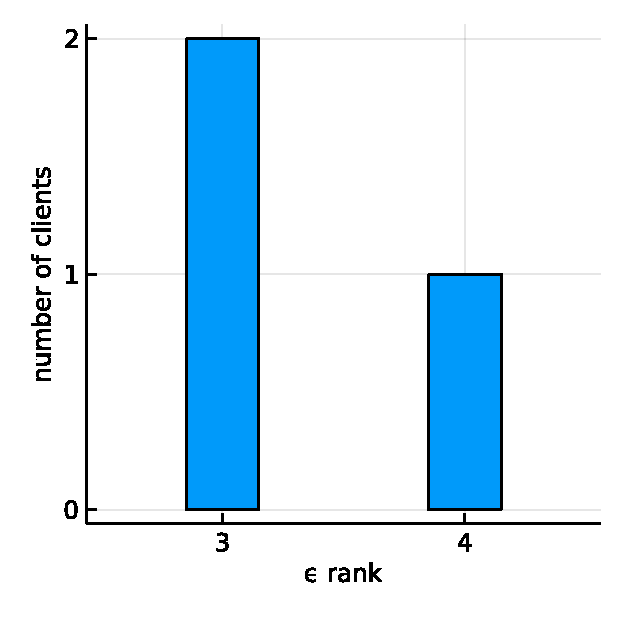
\includegraphics[width=\linewidth]{./figures/syn_embedding_matrix_adult.pdf}
      \caption{Adult dataset.}
      \label{fig:syn_embedding_matrix_adult}
    \end{subfigure}%
    \begin{subfigure}{.24\textwidth}
      \centering
      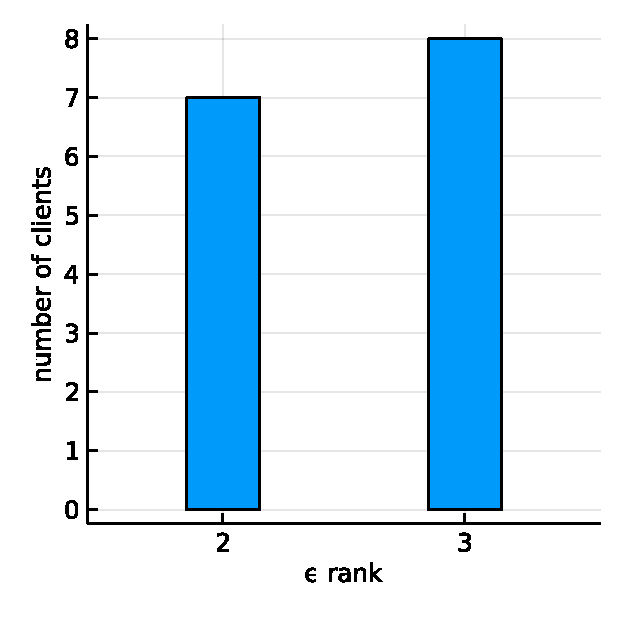
\includegraphics[width=\linewidth]{./figures/syn_embedding_matrix_web.pdf}
      \caption{Web dataset.}
      \label{fig:syn_embedding_matrix_web}
    \end{subfigure}
    \begin{subfigure}{.24\textwidth}
      \centering
      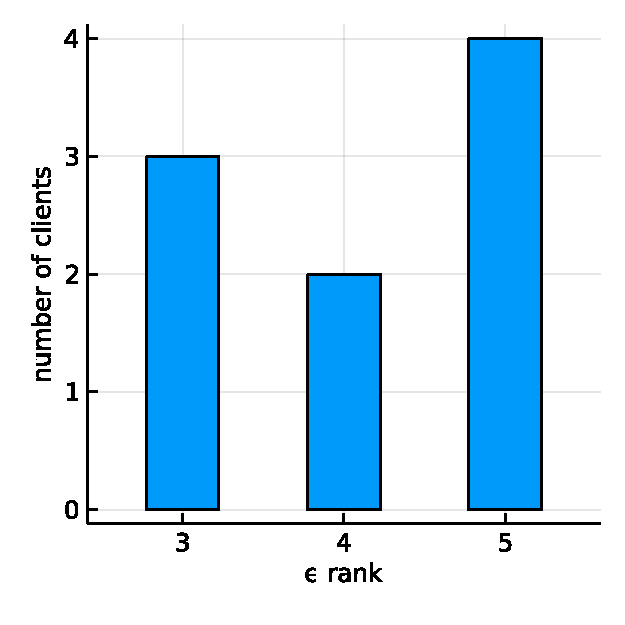
\includegraphics[width=\linewidth]{./figures/syn_embedding_matrix_covtype.pdf}
      \caption{Covtype dataset.}
      \label{fig:syn_embedding_matrix_covtype}
    \end{subfigure}
    \begin{subfigure}{.24\textwidth}
      \centering
      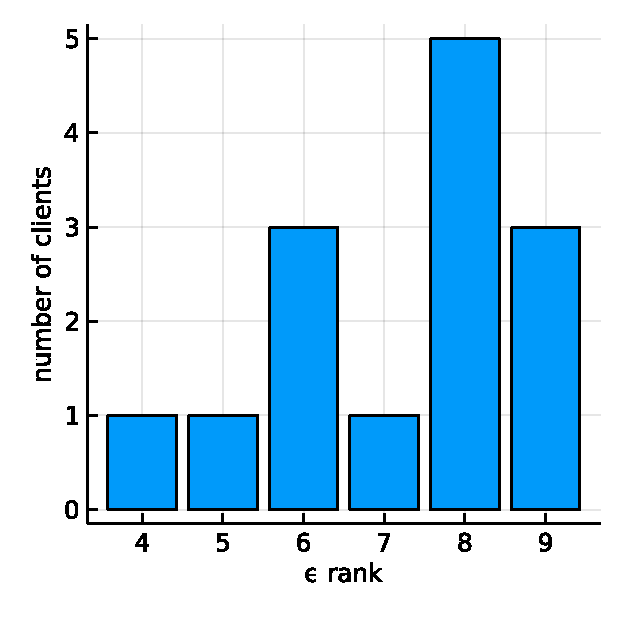
\includegraphics[width=\linewidth]{./figures/syn_embedding_matrix_rcv1.pdf}
      \caption{RCV1 dataset.}
      \label{fig:syn_embedding_matrix_rcv1}
    \end{subfigure}
    \caption{Approximated $\epsilon$-rank of embedding matrices.}
    \label{fig:syn_embedding_matrix}
\end{figure}

In this experiment, we numerically verify that the embedding matrices are approximately rank as described by Proposition~\ref{prop:low-rank}. Because we want to access the full embedding matrix, we set the batch size equal to the number of data points for all clients. The numbers of clients for the \emph{Adult}, \emph{Web}, \emph{Covtype} and \emph{RCV1} datasets are, respectively, $M = 3, 15, 9, 14$. Since computing the $\epsilon$-rank (\autoref{def:rank}) is NP-hard \cite{udell2019big}, we instead compute the rank of its truncated singular value decomposition as an approximation. More precisely, given a matrix $X \in \mathbb{R}^{m, n}$, let 
$\sigma_1 \geq \sigma_2 \geq \dots \geq \sigma_p$
be its ordered singular values, where $p = \min\{m,n\}$. Then given $\epsilon \in (0, 1)$, we define its approximated $\epsilon$-rank as 
\[\widehat \rank_\epsilon(X) = \max\{r \in [1, p] \mid \sigma_r \geq \epsilon \cdot \sigma_1\}.\]
We show a bar plot of the approximated $\epsilon$-rank of the embedding matrices in \autoref{fig:syn_embedding_matrix}, where $\epsilon=10^{-3}$, the x-axis represents the approximated $\epsilon$-rank and the y-axis represents number of clients. The plot shows that the embedding matrices have low approximated $\epsilon$-ranks for all the datasets.

\paragraph{Impact of feature heterogeneity}
\begin{figure}[t]
\begin{subfigure}{.24\textwidth}
  \centering
  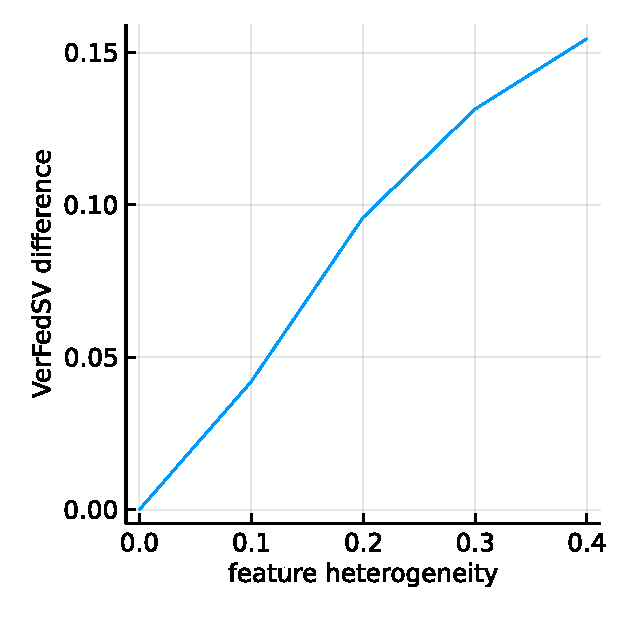
\includegraphics[width=\linewidth]{./figures/syn_similar_feature_adult.pdf}
  \caption{Adult dataset.}
  \label{fig:syn_similar_feature_adult}
\end{subfigure}%
\begin{subfigure}{.24\textwidth}
  \centering
  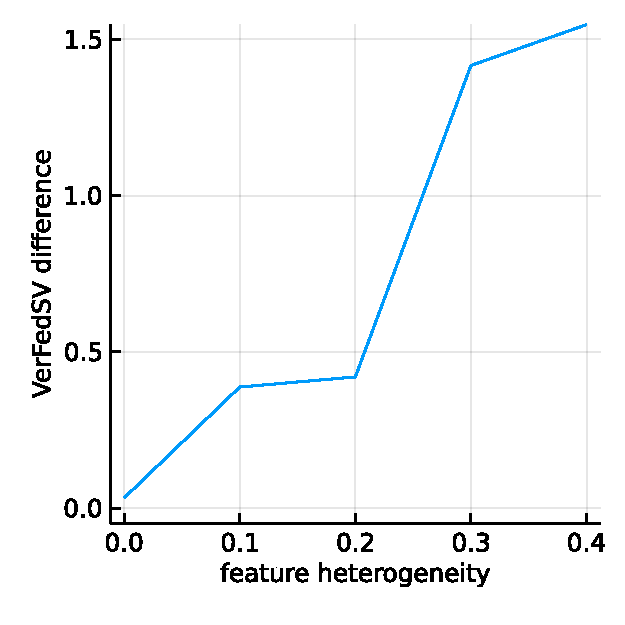
\includegraphics[width=\linewidth]{./figures/syn_similar_feature_web.pdf}
  \caption{Web dataset.}
  \label{fig:syn_similar_feature_web}
\end{subfigure} 
\begin{subfigure}{.24\textwidth}
  \centering
  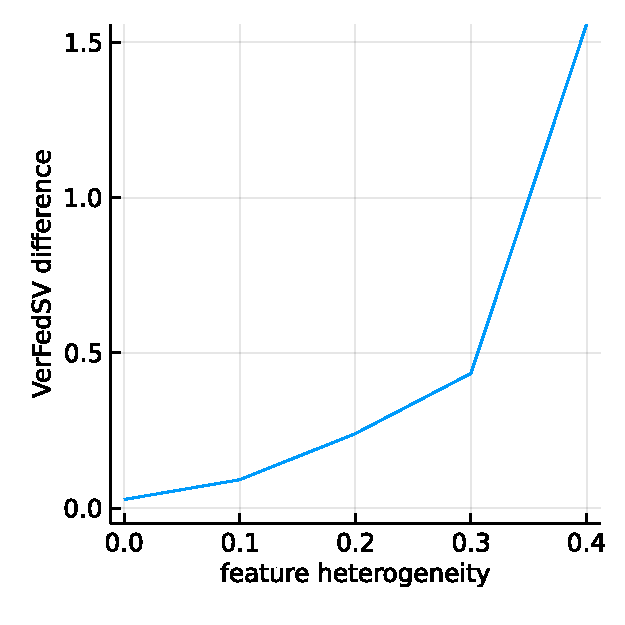
\includegraphics[width=\linewidth]{./figures/syn_similar_feature_covtype.pdf}
  \caption{Covtype dataset.}
  \label{fig:syn_similar_feature_covtype}
\end{subfigure}
\begin{subfigure}{.24\textwidth}
  \centering
  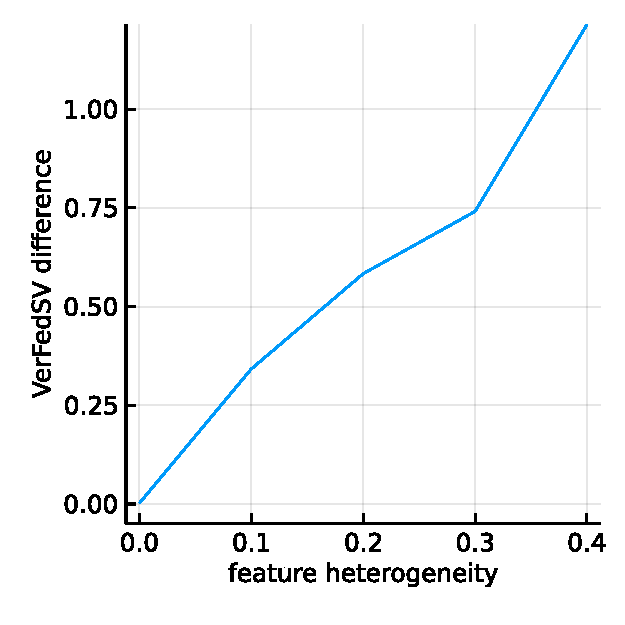
\includegraphics[width=\linewidth]{./figures/syn_similar_feature_rcv1.pdf}
  \caption{RCV1 dataset.}
  \label{fig:syn_similar_feature_rcv1}
\end{subfigure}
\caption{Relative VerFedSV difference vs feature heterogeneity.}
\label{fig:syn_similar_feature}
\end{figure}
In this experiment, we show that clients with similar features receive similar valuations under the synchronous setting. Besides the original clients, for each data set, we add 5 more clients whose features are identical to client 1 but with different level of perturbations. More precisely, for new client $i \in \{1,\dots,5\}$, we add white Gaussian noise to $(i-1)10\%$ percent of the local features, which we denote as the feature heterogeneity. Then we measure the relative difference between the original client 1 and the new clients, i.e., for any new client $i \in \{1,\dots,5\}$, let
$\texttt{diff}_i := \frac{|s - s_i|}{s}$,
where $s$ is the VerFedSV for the original client 1 and $s_i$ is the VerFedSV for the new client $i$. We show a plot of relative VerFedSV difference versus feature heterogeneity in \autoref{fig:syn_similar_feature}, where the numbers of clients for the \emph{Adult}, \emph{Web}, \emph{Covtype} and \emph{RCV1} datasets are, respectively, $M = 8, 20, 14, 19$. We can see that the relative VerFedSV difference is proportional to the feature heterogeneity. Besides, when the feature heterogeneity is equal to $0$, i.e., two clients have identical features, the relative VerFedSV difference is exactly $0$ for \emph{Adult} dataset, and is nearly $0$ for the \emph{Web}, \emph{Covtype} and \emph{RCV1} datasets, where the inexactness is due to the Monte Carlo sampling. 

\paragraph{VerFedSV for random feature}
In this experiment, we show that clients with randomly generated features receive low evaluations under synchronous setting. Besides the regular clients, for each data set, we add 5 more clients whose features are randomly generated according to different distributions. More precisely, for the new client $i \in \{1,\dots,5\}$, the features are generated from Gaussian distribution with mean equal to $i$ and variance equal to $i^2$. We show in the \autoref{tab:syn_random_feature} the percentage of the clients' VerFedSVs in the total sum of VerFedSVs, where the numbers of clients for the \emph{Adult}, \emph{Web}, \emph{Covtype} and \emph{RCV1} datasets are, respectively, $M = 8, 20, 14, 19$. As we can see from the table, regardless of the distributions, clients with randomly generated features receive much lower valuations than the regular clients for all the datasets. 
\begin{table}[t]
    \centering
    \begin{tabular}{ccccc}
    \toprule
                         & Adult & Web   & Covtype  & RCV1 \\ \midrule
     all regular clients & 99.88 & 99.73 & 97.77    & 93.84\\
     artificial client 1 & 0.01  & 0.02  & 0.39     & 1.86 \\
     artificial client 2 & 0.05  & 0.06  & 0.57     & 0.43\\
     artificial client 3 & 0.03  & 0.06  & 0.91     & 2.37\\
     artificial client 4 & 0.01  & 0.07  & 0.36     & 0.31\\
     artificial client 5 & 0.02  & 0.06  & 0.01     & 1.18\\
    \bottomrule
    \end{tabular}
    \caption{Percentage of clients' VerFedSVs in the total sum of VerFedSVs (synchronous setting).}
    \label{tab:syn_random_feature}
\end{table}

\subsection{Asynchronous Vertical Federated Learning} \label{sec:8.8.3}
In this set of experiments, we adapt VerFedSV with asynchronous VFL algorithms. We show that VerFedSV not only satisfies the fairness property under asynchronous setting (\autoref{thm:fair}), but can also reflect how frequently clients report (\autoref{prop:asyn_diff_fre}). More specifically, during the training, we let clients to communicate with server at different frequencies. For all the datasets, we asynchronously train the model for $20$ seconds and do the valuation every $0.04$ seconds, i.e., there are $T = 500$ contribution valuation time points (\autoref{def:vertical_fedsv}). 

\paragraph{Impact of communication frequency}

\begin{figure}[t]
\begin{subfigure}{.24\textwidth}
  \centering
  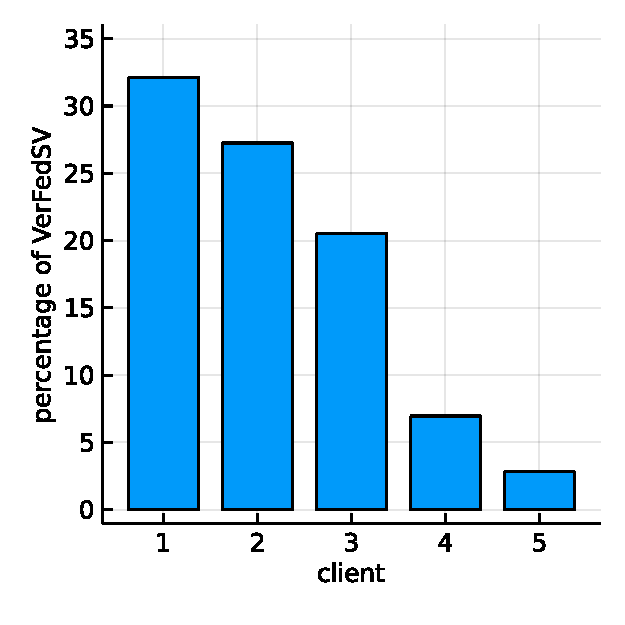
\includegraphics[width=\linewidth]{./figures/asyn_same_features_adult.pdf}
  \caption{Adult dataset.}
  \label{fig:asyn_same_feature_adult}
\end{subfigure}%
\begin{subfigure}{.24\textwidth}
  \centering
  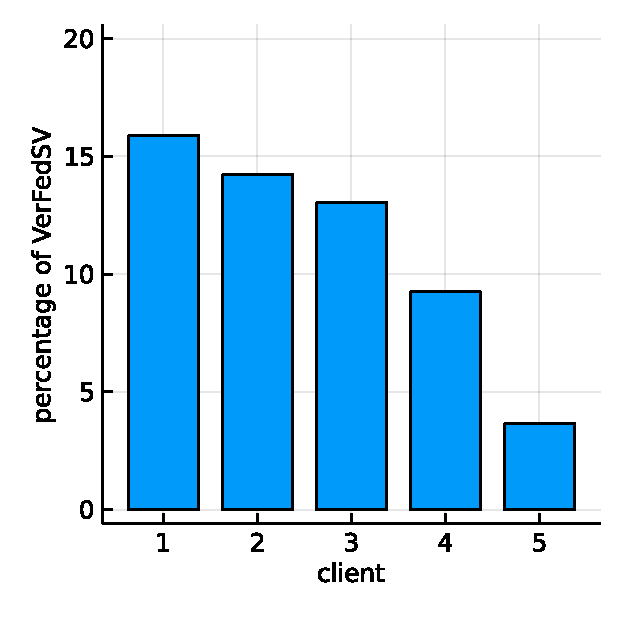
\includegraphics[width=\linewidth]{./figures/asyn_same_features_web.pdf}
  \caption{Web dataset.}
  \label{fig:asyn_same_feature_web}
\end{subfigure} 
\begin{subfigure}{.24\textwidth}
  \centering
  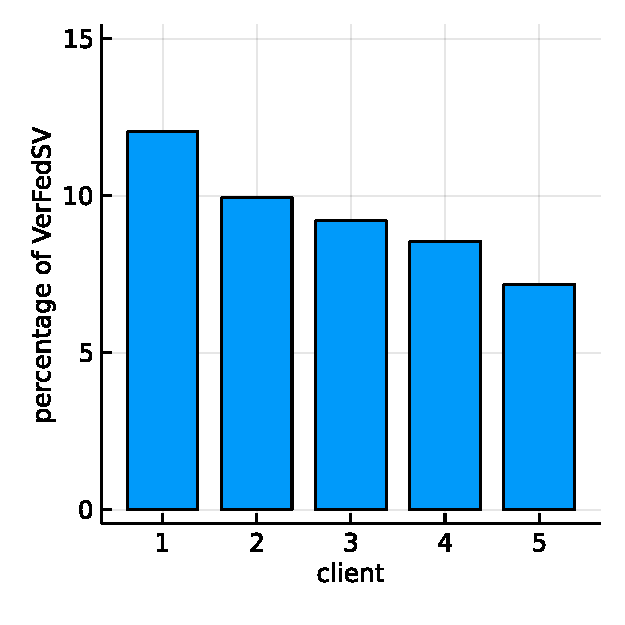
\includegraphics[width=\linewidth]{./figures/asyn_same_features_covtype.pdf}
  \caption{Covtype dataset.}
  \label{fig:asyn_same_feature_covtype}
\end{subfigure}
\begin{subfigure}{.24\textwidth}
  \centering
  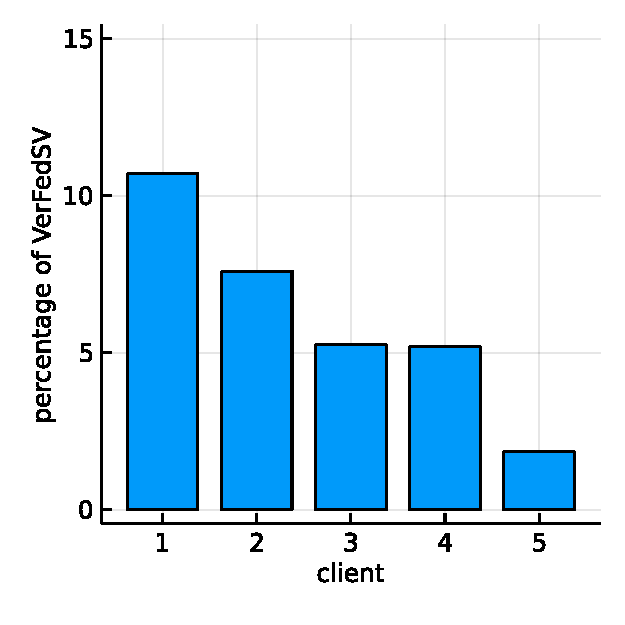
\includegraphics[width=\linewidth]{./figures/asyn_same_features_rcv1.pdf}
  \caption{RCV1 dataset.}
  \label{fig:asyn_same_feature_rcv1}
\end{subfigure}
\caption{VerFedSVs for clients with different communication frequencies.}
\label{fig:asyn_same_feature}
\end{figure}

In this experiment, we show that clients with higher communication frequency receive higher valuation. Besides the original clients, for each data set, we add 5 more clients whose features are identical to client 1 but with different level of communication frequencies. More precisely, the new client $i \in \{1,\dots,5\}$ communicates with the server every $0.01i$ seconds, i.e., the new client 1 has the highest communication frequency and the new client $5$ has the lowest. We show a plot in \autoref{fig:asyn_same_feature} of the percentage of the new clients' VerFedSVs in the total sum of VerFedSVs, where the numbers of clients for the \emph{Adult}, \emph{Web}, \emph{Covtype} and \emph{RCV1} datasets are, respectively, $M = 8, 20, 14, 19$. We can see that the percentage of VerFedSV is proportional to the communication frequency. 

\paragraph{VerFedSV for random feature}
In this experiment, we show that clients with randomly generated features receive low evaluations regardless of their communication frequencies. Besides the regular clients, for each data set, we add 5 more clients whose features are randomly generated according to standard Gaussian distribution. They have communication frequencies such that the new client $i \in \{1,\dots,5\}$ communicates with the server every $0.01i$ seconds. We show in \autoref{tab:asyn_random_feature} the percentage of the clients' VerFedSVs in the total sum of VerFedSVs, where the numbers of clients for the \emph{Adult}, \emph{Web}, \emph{Covtype} and \emph{RCV1} datasets are, respectively, $M = 8, 20, 14, 19$. Regardless of the communication frequencies, the clients with randomly generated features receive much lower valuations than the regular clients for all the datasets.
\begin{table}[t]
    \centering
    \begin{tabular}{ccccc}
    \toprule
                         & Adult & Web   & Covtype  & RCV1\\ \midrule
     all regular clients & 97.91 & 98.39 & 98.57    & 91.90\\
     artificial client 1 & 0.93  & 0.26  & 0.35     & 1.66\\
     artificial client 2 & 0.06  & 0.31  & 0.21     & 1.75\\
     artificial client 3 & 0.33  & 0.36  & 0.22     & 1.64\\
     artificial client 4 & 0.43  & 0.40  & 0.25     & 1.50\\
     artificial client 5 & 0.35  & 0.28  & 0.39     & 1.54\\
    \bottomrule
    \end{tabular}
    \caption{Percentage of clients' VerFedSVs in the total sum of VerFedSVs (asynchronous setting).}
    \label{tab:asyn_random_feature}
\end{table}

\subsection{Effectiveness of VerFedSV} \label{sec:8.8.4}
We evaluate the effectiveness of VerFedSV in both the synchronous and asynchronous VFL settings. In other words, we test whether VerFedSV can reflect the importance of clients' local features. We set all clients to have the same communication frequency to eliminate the impact of unbalanced local computational resources. We choose SHAP~\cite{lundberg2017unified} as the baseline, which is a widely-used metric for measuring feature importance in machine learning. More specifically, we first use SHAP to compute the importance scores of all the features, and then for each client, we ensemble the scores for all the local features. Note that SHAP cannot be directly used in the VFL task, as it requires access to all the local datasets and models and violates the VFL settings. So here we just use it as a reference. We use the Kendall's rank correlation (KRC)~\cite{kendall1938new} to measure the similarity between the orderings of the scores of SHAP and VerFedSV. As a by-product, we also show the similarity between the scores of VerFedSV in the synchronous and asynchronous settings. We show in \autoref{tab:comparasion_shap} the KRCs between the results of SHAP and VerFedSV, where $\corr$ denotes the KRC, $\svshap$ denotes the results from SHAP, $\svsyn$ and $\svasyn$, respectively, denote the results from VerFedSV in the synchronous and asynchronous settings, and the numbers of clients for the \emph{Adult}, \emph{Web}, \emph{Covtype} and \emph{RCV1} datasets are, respectively, set to $M = 3, 15, 9, 14$. Note that KRC returns a value in $[-1, 1]$, where ``$1$'' means two input score lists have the identical ranking and ``$-1$'' means the rankings are exactly reverted. The KRC between SHAP and VerFedSV are all greater than $0.6$. The results indicate that VerFedSV can indeed capture the feature importance well. Moreover, the KRC between $\svsyn$ and $\svasyn$ are all greater than 0.8. The results indicate that VerFedSV is consistent under both synchronous and asynchronous settings.

\begin{table}[t]
    \centering
    \begin{tabular}{ccccc}
    \toprule
                                & Adult & Web   & Covtype   & RCV1\\ \midrule
    $\corr(\svshap, \svsyn)$    & 1.0   & 0.73  & 0.94      & 0.65\\
    $\corr(\svshap, \svasyn)$   & 1.0   & 0.69  & 0.89      & 0.63\\
    $\corr(\svsyn, \svasyn)$    & 1.0   & 0.80  & 0.94      & 0.80\\
    \bottomrule
    \end{tabular}
    \caption{Kendall's rank correlation between the results of SHAP and VerFedSV's.}
    \label{tab:comparasion_shap}
\end{table}

\section{Insights} \label{sec:8.9}
In this paper, we propose a contribution valuation metric called vertical federated Shapley value (VerFedSV) for vertical federated learning (VFL). We demonstrate both theoretically and empirically that VerFedSV satisfies many desirable properties for fairness and is quite adaptable such that it can be applied under both synchronous and asynchronous VFL settings. 

There are a few interesting directions for future work.  For example, there is an interesting insight from the experiments that deserves future research.  We notice that when we keep adding clients with identical features, the total of the VerFedSV increases. This may suggest that some clients may ``cheat'' by constructing new clients with identical features so that they can receive unjustifiable rewards in the end. The issue can be resolved under the synchronous setting, for example, by checking the similarity between uploaded embeddings from clients. However, it seems there is no simple solution to resolve this issue under the asynchronous setting. 

\section{Proofs}

\subsection{Proof for Theorem 1}
\begin{proof}
    We notice that the VerFedSV can be expressed as 
    \begin{align*}
        s_m &= \frac{1}{MT}\sum_{t=1}^T\sum_{S \subseteq [M] \setminus \{m\}} \frac{1}{\binom{M-1}{|S|}} [U_t(S\cup\{m\}) - U_t(S)]\\
        &= \frac{1}{M}\sum_{S \subseteq [M] \setminus \{m\}} \frac{1}{\binom{M-1}{|S|}} \left[\frac{1}{T}\sum_{t=1}^T U_t(S\cup\{m\}) - \frac{1}{T}\sum_{t=1}^T U_t(S)\right]\\
        &= \frac{1}{M}\sum_{S \subseteq [M] \setminus \{m\}} \frac{1}{\binom{M-1}{|S|}} \left[U(S\cup\{m\}) - U(S)\right],
    \end{align*}
    which matches the expression for classical Shapley value. The result then follows. 
\end{proof}

\subsection{Proof for Proposition 1}
\begin{proof}
    It is evident that $\rank_\epsilon(\mathcal{H}^m) \leq \rank(\mathcal{H}^m) \leq d_m$ for all $m \in [M]$. So we only need to prove the remaining two upper bounds. First, we consider the difference between successive rows of the embedding matrix $\mathcal{H}^m$. For any $t \in [T-1]$ and $i \in [N]$, 
    \begin{align*}
        |\mathcal{H}^m_{t, i} - \mathcal{H}^m_{t+1, i}| &= |(h_i^m)^{(t)} - (h_i^m)^{(t+1)}|
        \\&= |\langle \theta_m^{(t)}, x^m_i\rangle - \langle \theta_m^{(t+1)}, x^m_i\rangle|
        \\&= |\langle \theta_m^{(t)} - \theta_m^{(t+1)}, x^m_i\rangle|
        \\&= \left|\langle \frac{\eta^{(t)}}{|B^{(t)}|}\sum_{j\in B^{(t)}} g_j^{(t)} x_j^m , x^m_i\rangle\right|
        \\&\leq \eta^{(t)}L.
    \end{align*}
    Thus, we obtain an upper bound on the $\rank_\epsilon(\mathcal{H}^m)$ by 
    \begin{align*}
        \rank_\epsilon(\mathcal{H}^m) &\leq \left\lceil \frac{1}{\epsilon} \sum_{t=1}^{T-1} \big\|\mathcal{H}^m[t,:] - \mathcal{H}^m[t+1, :]\big\|_{\max} \right\rceil \\
        &\leq \left\lceil \frac{L}{\epsilon} \sum_{t=1}^{T-1}\eta^{(t)} \right\rceil\\
        &\leq \left\lceil \frac{L\log(T)}{\epsilon} \right\rceil.
    \end{align*}
    Next, we consider the difference between any two columns of the embedding matrix $\mathcal{H}^m$. For any $t \in [T]$ and $i,j\in[N]$, we have 
    \begin{align*}
        |\mathcal{H}^m_{t, i} - \mathcal{H}^m_{t, j}| &= |(h_i^m)^{(t)} - (h_j^m)^{(t)}|
        \\&= |\langle \theta_m^{(t)}, x^m_i\rangle - \langle \theta_m^{(t)}, x^m_j\rangle|
        \\&\leq \|\theta_m^{(t)}\|\cdot\|x^m_i - x^m_j\|.
    \end{align*}
    It follows that 
    \[\|\mathcal{H}^m[:,i] - \mathcal{H}^m_{t, j}\|_{\max} \leq \max_{t \in [T]}\|\theta_m^{(t)}\|\cdot\|x^m_i - x^m_j\|.\]
    Let $\gamma^m = \max_{t \in [T]}\|\theta_m^{(t)}\|$ and $\mathcal{N}$ be an $\frac{\epsilon}{\gamma^m}$-net for $\{x^m_i : i \in [N]\}$. We can thus conclude that 
    \[\rank_\epsilon(\mathcal{H}^m) \leq |\mathcal{N}|.\]
    By definition of the covering number, it follows that 
    \[\rank_{\epsilon}(\mathcal{H}^m) \leq \mathcal{N}\left(\{x^m_i: i \in [N]\}, \frac{\epsilon}{\gamma^m}\right).\]
\end{proof}

\section{Proof for Proposition 2}
\begin{proof}
    Define $U,\hat U: 2^{[M]}\to\mathbb{R}$ by 
    \[U(S) := \frac{1}{T}\sum_{t=1}^T U_t(S) \quad\text{and}\quad \hat U(S) := \frac{1}{T}\sum_{t=1}^T \hat U_t(S).\]
    For any $S \subset [M]$, we know that 
    \begin{align*}
        &~|U(S) - \hat U(S)| \\
        \leq~&~\frac{1}{NT}\sum_{t=1}^T\sum_{i=1}^N \left|f\left( \sum_{m=1}^M \mathcal{H}_{t-1, i}^m; y_i\right) - f\left( \sum_{m=1}^M (w^m_{t-1})^\intercal h^m_i; y_i\right)\right| \\
        &~+ \frac{1}{NT}\sum_{t=1}^T\sum_{i=1}^N \bigg|f\left( \sum_{m\in S} \mathcal{H}_{t, i}^m + \sum_{m\notin S} \mathcal{H}_{t-1, i}^m; y_i\right) \\
        &~- f\left( \sum_{m\in S} (w^m_{t})^\intercal h^m_i + \sum_{m\notin S} (w^m_{t-1})^\intercal h^m_i; y_i\right)\bigg|\\
        \leq~&~\frac{G}{NT}\sum_{t=1}^T\sum_{i=1}^N \left|\sum_{m=1}^M \mathcal{H}_{t-1, i}^m -  \sum_{m=1}^M (w^m_{t-1})^\intercal h^m_i\right|\\
        &~+ \frac{G}{NT}\sum_{t=1}^T\sum_{i=1}^N \bigg|\left( \sum_{m\in S} \mathcal{H}_{t, i}^m + \sum_{m\notin S} \mathcal{H}_{t-1, i}^m\right) \\ 
        &~- \left( \sum_{m\in S} (w^m_{t})^\intercal h^m_i + \sum_{m\notin S} (w^m_{t-1})^\intercal h^m_i\right)\bigg| \leq GM\epsilon.
    \end{align*}
    Then we can obtain a bound on $|s_m - \hat s_m|$ by 
    \begin{align*}
        ~&~|s_m - \hat s_m| \\
        \leq ~&~ \frac{1}{M}\sum_{S \subseteq [M] \setminus \{m\}} \frac{1}{\binom{M-1}{|S|}} \left|U(S\cup\{m\}) - \hat U(S\cup\{m\})\right| + \left|U(S) - \hat U(S)\right|\\
        \leq ~&~ 2G\epsilon.
    \end{align*}
\end{proof}

\subsection{Proof for Proposition 3}
\begin{proof}
    We know that $\theta_1^*$ and $\theta_2^*$ are the optimal variables for the following convex optimization problem 
    \[\min_{\theta_1, \theta_2}\enspace \frac{1}{N}\sum_{i=1}^N f(\langle\theta_1, x_i\rangle + \langle\theta_2, x_i\rangle; y_i) = g(\theta_1 + \theta_2).\]
    Since $\theta^*$ is the unique minimizer for $g(\theta)$, it follows that $\theta_1^*$ and $\theta_2^*$ must satisfy $\theta_1^* + \theta_2^* = \theta^*$. Denote $d_1^{(t)}$ as the update for $\theta_1$ at the $t$th iteration and $d_2^{(t)}$ as the update for for $\theta_2$ at the $t$th iteration. By the construction, we know that 
    \[\mathbb{E} \left[ \sum_{t=1}^\infty ( d_1^{(t)} + d_2^{(t)} ) \right] = \theta^* \enspace\text{and}\enspace \mathbb{E}\left[ \sum_{t=1}^\infty d_2^{(t)} \right] = \rho \mathbb{E}\left[ \sum_{t=1}^\infty d_1^{(t)} \right].\]
    Therefore
    \[
        \mathbb{E}[\theta_1^*] = \mathbb{E}\left[ \sum_{t=1}^\infty d_1^{(t)} \right] = \frac{1}{1+\rho} \theta^* \enspace\text{and}\enspace \mathbb{E}[\theta_2^*] = \mathbb{E}\left[ \sum_{t=1}^\infty d_2^{(t)} \right] = \frac{\rho}{1+\rho} \theta^*.
    \]
    Now we consider VerFedSV. By the definition, we have 
    \[\mathbb{E}[s_1 - s_2] = 2\left[g\left(\frac{\rho}{1+\rho}\theta^*\right) - g\left(\frac{1}{1+\rho}\theta^*\right)\right].\]
    Define $h:[0,1]\to\mathbb{R}$ as $h(\lambda) = g(\lambda \theta^*)$. Since $g$ is $\mu$-strongly convex and $\theta^*$ is the unique minimizer, it follows that $h$ is $\mu\|\theta^*\|^2$-strongly convex and is monotonically non-increasing on $[0,1]$. Thus, we can conclude that 
    \[\mathbb{E}[s_1] \geq \mathbb{E}[s_2] + 2\left[h\left(\frac{\rho}{1+\rho}\right) - h\left(\frac{1}{1+\rho}\right)\right] \geq \mathbb{E}[s_2] + \mu\left(\frac{1-\rho}{1+\rho}\right)^2\|\theta^*\|^2.\]
\end{proof}